\chapter{Experimentación y evaluación}
%-----------------------------------------------
% 5.1 Scientific workflows
%-----------------------------------------------
\section{Experimentos computacionales}\label{s5.1}

Para validar nuestra propuesta y su aplicación en el contexto de workflows científicos, se ha seleccionado un subconjunto de workflows y WMSs. 
El subconjunto ha sido seleccionado bajo los criterio de: nivel de utilización de WMS, el lenguaje utilizado en él, y disponibilidad de los materiales del workflow.
Los materiales deben incluir los datos de ingresos que permitan reproducir de forma completa el workflow, documentación, resultados o anotaciones. Además nos debe permitan comparar los resultados de nuestro ambientes resultantes.

Para cada WMS, hemos construimos una imagen estándar. En consecuencia, un investigador puede importar esta imagen e instalar los componentes de software relacionados con el workflow.
Esto se puede conseguir utilizando la instrucción FROM de Dockerfile. Por ejemplo, el workflow de SoyKB utiliza el workflow manager system: Pegasus. Por lo tanto, la imagen SoyKb importa la imagen Pegasus.
Para entender los requisitos del workflow, nosotros inspeccionamos la documentación disponible y las anotaciones generadas por WICUS \cite{santana2017reproducibility}.
En caso que el WMSs no distribuya su software utilizando Docker, se construye las imágenes, los archivos necesarios como configuraciones y el DeploymentPlan (Dockerfile). Estos archivos están disponibles en nuestros repositorios para cada flujo de trabajo. \footnote{https://github.com/dockerpedia}.
Además, cada DeploymentFile incluye información sobre la imagen utilizando el estándar de la Open Container Initiative \footnote{\url{https://www.opencontainers.org/}}. 

\subsection{Pegasus}

Pegasus~\cite{} es un WMS capaz de gestionar flujos de trabajo compuestos por millones de tareas, registrando datos sobre la ejecución y resultados intermedios. 
Cuando se producen errores, Pegasus intenta recuperarse cuando es posible reintentando tareas, reintentando todo el flujo de trabajo, proporcionando puntos de control a nivel de flujo de trabajo, re-mapeando partes del flujo de trabajo, probando fuentes de datos alternativas para la puesta a disposición de los datos y, cuando todo lo demás falla, proporcionando un flujo de trabajo de rescate que contiene sólo una descripción del trabajo que queda por hacer. Limpia el almacenamiento a medida que se ejecuta el flujo de trabajo, de modo que los flujos de trabajo de datos intensivos tengan suficiente espacio para ejecutarse en recursos limitados por el almacenamiento]. Pegasus lleva un registro de lo que se ha hecho (procedencia), incluyendo las ubicaciones de los datos utilizados y producidos, y qué software se utilizó con qué parámetros.
Pegasus lee las descripciones del flujo de trabajo de los archivos DAX. El término DAX" es la abreviatura de "Directed Acyclic Graph in XML". DAX es un formato de archivo XML que tiene sintaxis para expresar trabajos, argumentos, archivos y dependencias. Para crear un DAX es necesario escribir código para un generador de DAX. 
Pegasus opcionalmente utiliza en HTCondor como administrador de tareas. Por lo tanto, construimos dos versiones para la imagen de Pegasus; una versión tiene ins
talado el paquete condor y otra sin él. La justificación de decisión recae en permitir a los científicos utilizar una imagen simple si es necesario.
El paquete Pegasus ha sido obtenido del repositorio oficial~\footnote{\url{http://download.pegasus.isi.edu/wms/download/debian}}.
Los principales requisitos de pegasus son: Java,  (la versión Java depende de la versión pegasus), python y perl. La figura \ref{fig:pegasus-deps.pdf} muestra las dependencias especificadas tanto por el sistema de paquetes o documentación.

\begin{figure}[t]
\centering
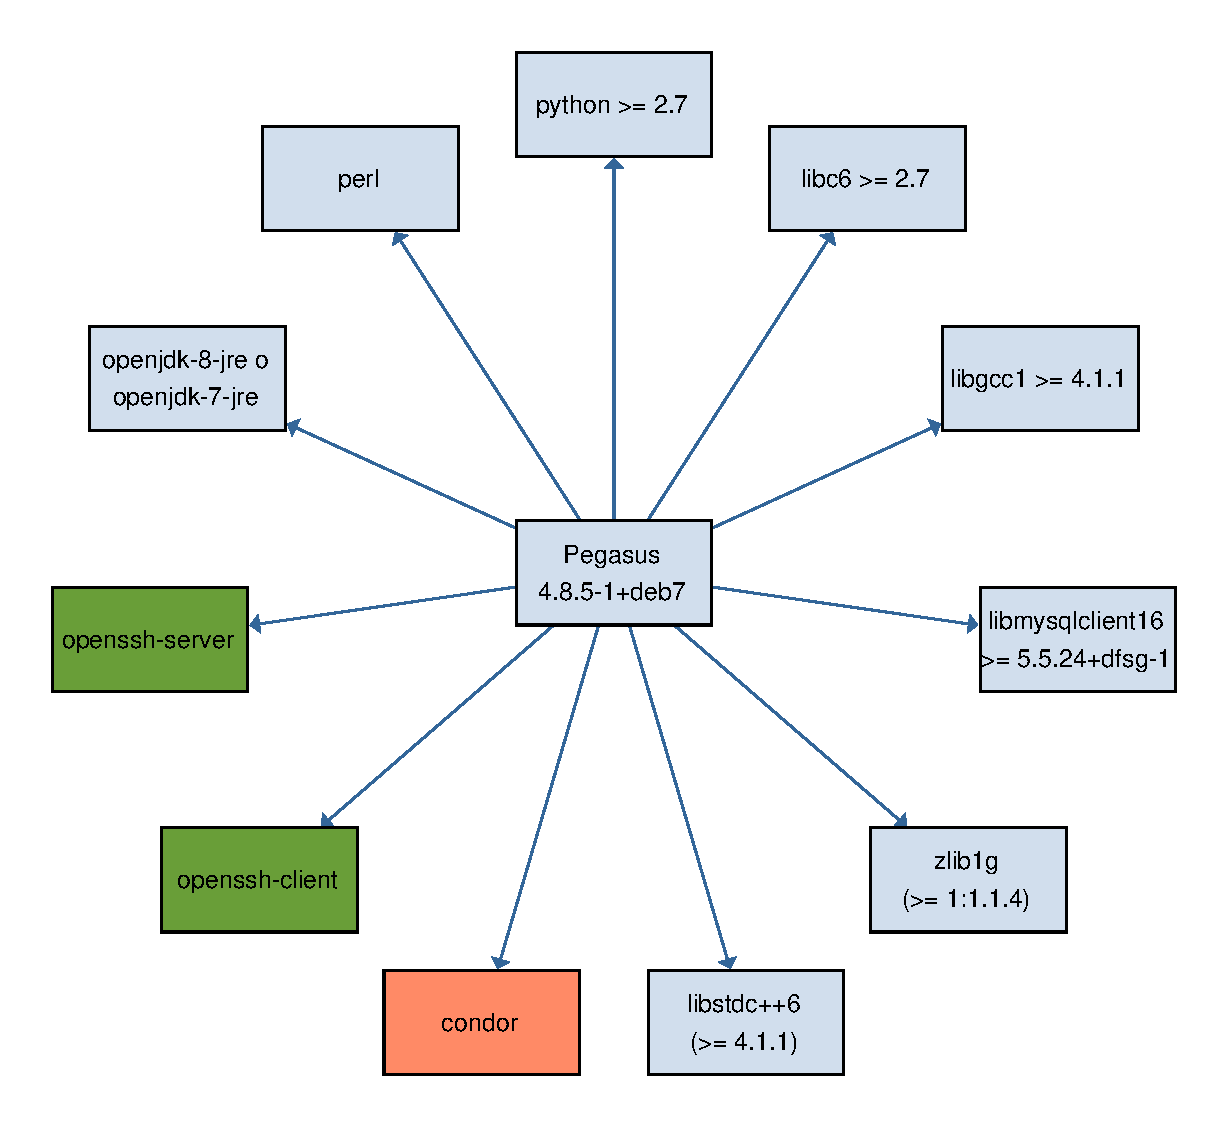
\includegraphics[width=.5\textwidth]{Figures/pegasus-deps}
\caption{Dependencias de Pegasus. En azul: dependencias necesarias y especificadas en el sistema de paquetes. En verde: necesarias pero no especificadas en el sistema de paquetes. En naranjas: dependencias recomendadas}\label{fig:pegasus-deps}
\end{figure}

Las imágenes se encuentran disponibles en DockerHub~\footnote{\url{https://hub.docker.com/r/dockerpedia/pegasus_workflow_images/}}

\subsubsection{Soybean Knowledge Base}

El workflow SoyKB (Soybean Knowledge Base) \cite{joshi2012soybean} permite realizar un proceso de re-secuencia de germoplasma de la soya, ésta ha sido seleccionada para estudiar rasgos como aceites, proteina, resistencia de los nematodos del quiste de la soya y resistencia al estrés.
Pegasus presenta un workflow que implementa polimorfismo de nucleótido único (SNP), la operación insertar/remover (indel) de la base del genoma de un organismo y una análisis utilizando el software GATK \footnote{\url{https://software.broadinstitute.org/gatk/}}
La figura \ref{fig:soykb} muestra   una representación gráfica del workflow, donde se realiza un análisis en paralelo de las muestras para que sean alineadas con el genoma de referencia y se identifique los indels y SNPs. Luego fusiona y filtra los resultados. 

\begin{figure}[t]
\centering
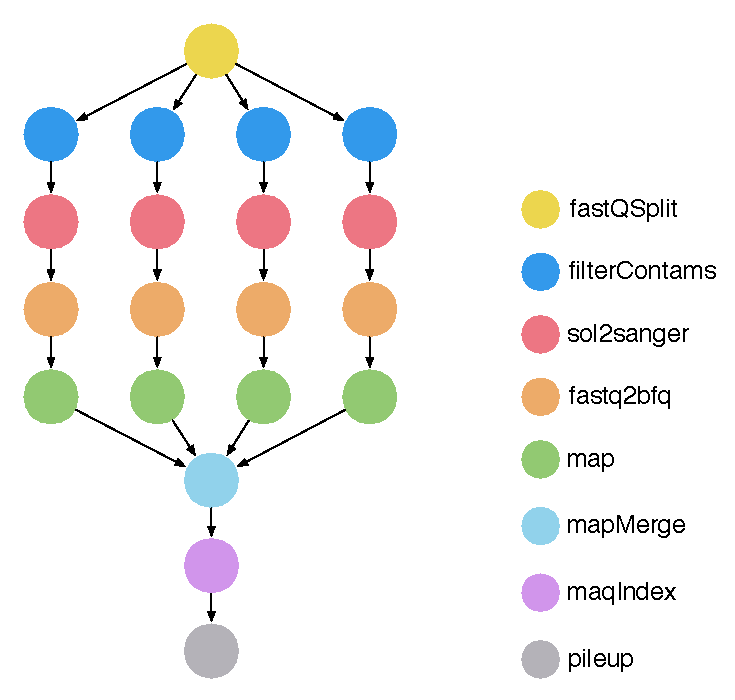
\includegraphics[width=.5\textwidth]{Figures/workflow-genome}
\caption{Representación entregada por Pegasus del workflow SoyKB.}\label{fig:soykb}
\end{figure}

Los componentes de software utilizados por SoyKB se clasifican en dos tipos: propio (en amarillo) y de terceros (en verde). Los componentes principales son: bwa, gatk y bwa y el software de tercero java-1.7.0

\begin{figure}[t]
\centering
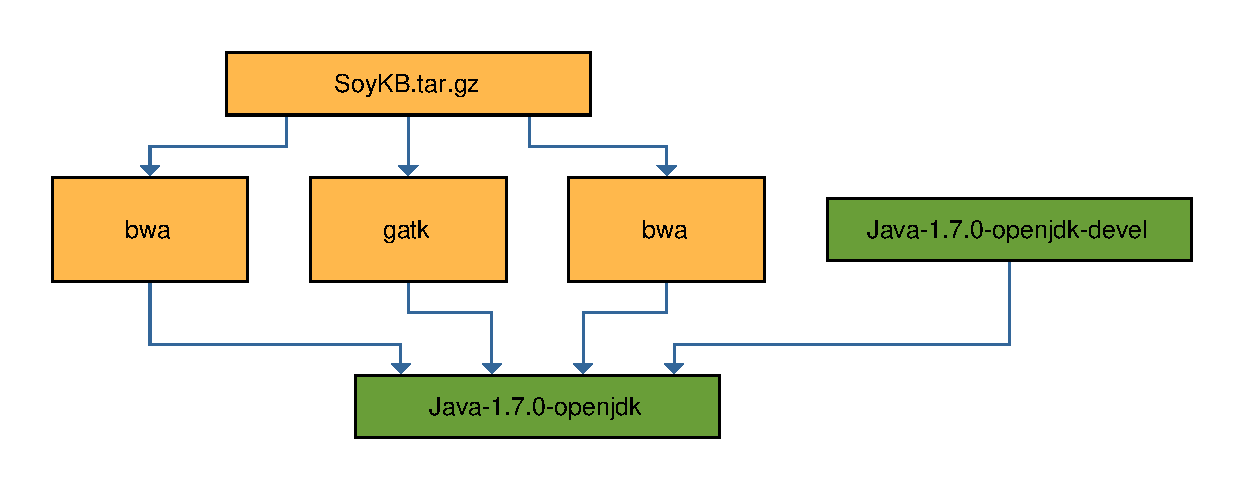
\includegraphics[width=.8\textwidth]{Figures/soykb-deps}
\caption{Dependencias de SoyKb. En amarillo: software propio y en verde software de terceros}\label{fig:modflow} 
\end{figure}

La evaluación de los resultados se realizó de forma manual al igual que en \cite{santana2017reproducibility} debido a los pasos aleatorios del workflow. La metodología fue una verificación manual de la estructura de los resultados, el tamaño de los archivos, número de líneas y la inexistencia de errores.

\subsubsection{Montage}

Montage es un set de herramientas creadas por \textit{NASA Infrared Processing and Analysis Center (IPAC)}, permitiendo generar bajo demanda mosaicos de imágenes astronómicas personalizadas, a partir de archivos de entrada que cumplen con el estándar del Sistema de Transporte Flexible de Imágenes (FITS) y que contienen datos de imágenes registrados en proyecciones que cumplen con los estándares del Sistema Mundial de Coordenadas (WCS).

La figura \ref{fig:montage} entregada por Pegasus ilustra el workflow Montage. Cada uno de los nodos de la figura es un software binario que generan la imagen final.

Debido a que el software es un binario, no se encuentra empaquetado. Por lo tanto fue descargado de la fuente. La dirección de descarga se encuentran en el plan de despliegue \footnote{\url{https://github.com/dockerpedia/montage/blob/master/Dockerfile}}. 

\begin{figure}[t]
\centering
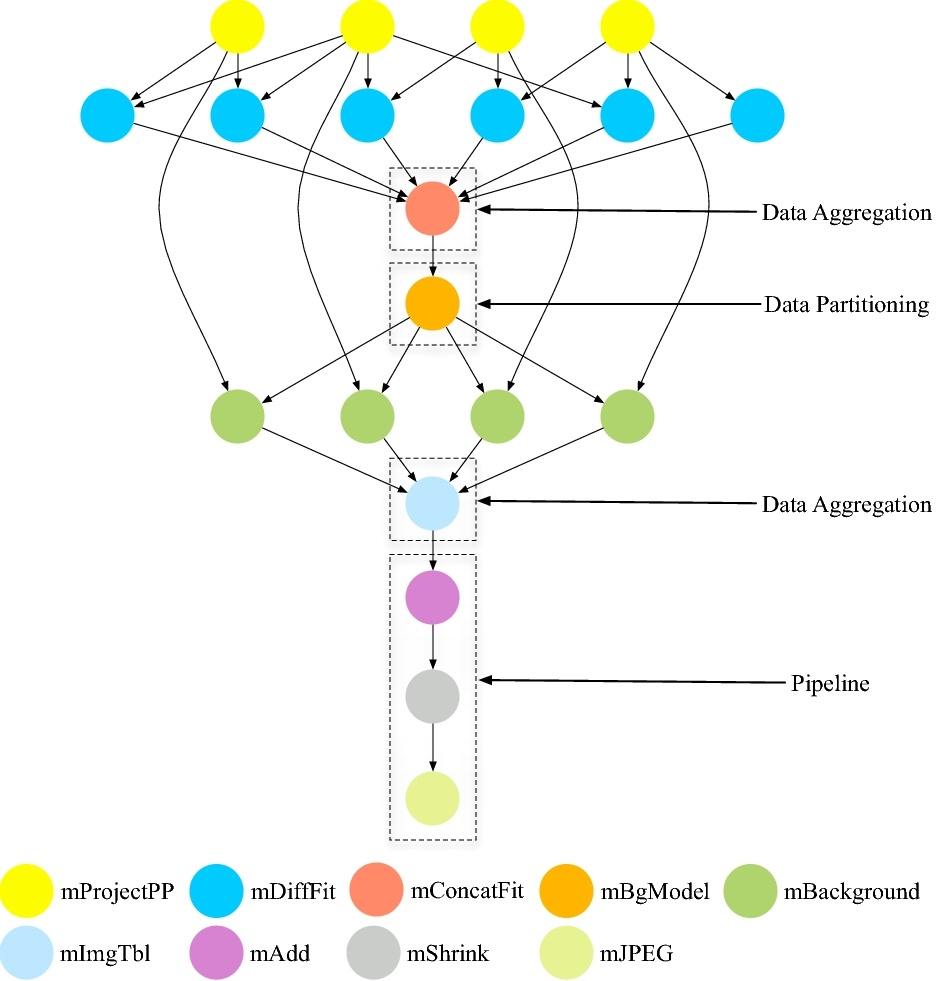
\includegraphics[width=.5\textwidth]{Figures/montage}
\caption{Representación entregada por Pegasus del workflow Montage.}\label{fig:montage}
\end{figure}

En el caso de Montage, se produce una imagen como salida, por ello utilizamos la herramienta de hash perceptual \footnote{\url{http://phash.org}} para realizar la comparación entre la imagen reproducida (imagen del cielo de 0,1 grados) frente a la original.
Como resultado, se obtiene un factor de similitud de 1,0 (más de 1,0) con un umbral de 0,85.
Las figuras \ref{fig:montage-wicus} y \ref{montage-mosorio} muestran las imágenes resultantes y los archivos resultantes en formato FITS se encuentran en nuestro repositorio \footnote{\url{https://github.com/dockerpedia/montage_results}}. 

\begin{figure*}[h]
    \centering
    \begin{subfigure}[b]{0.4\textwidth}
         \centering
         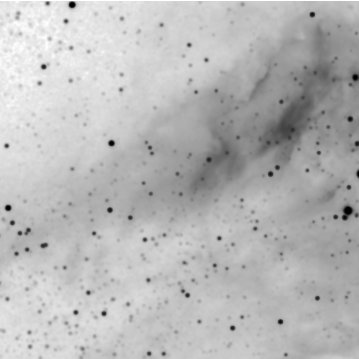
\includegraphics[width=\textwidth]{Figures/montage-original}
         \caption{Resultados originales obtenidos desde WICUS}
         \label{fig:montage-wicus}
     \end{subfigure}
         ~ 
	    \begin{subfigure}[b]{0.4\textwidth}
         \centering
         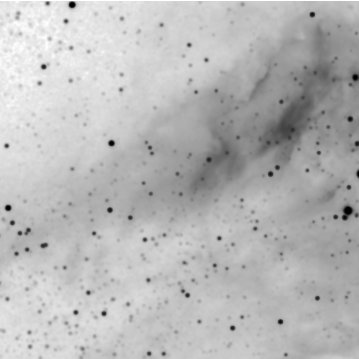
\includegraphics[width=\textwidth]{Figures/montage-mosorio}
         \caption{Resultados reproducidos por nuestra propuesta}
         \label{fig:montage-mosorio}
     \end{subfigure}
        \caption{Los resultados obtenidos con el nuevo ambiente son iguales}
        \label{fig:montage-results}
\end{figure*}



\subsection{dispel4py}

dispel4py ~\cite{} es una biblioteca Python para describir workflow. Describe flujos de trabajo abstractos para aplicaciones intensivas, que luego se traducen y ejecutan en plataformas distribuidas (por ejemplo, Apache Storm, clusters MPI, etc.).
El paquete dispel4py ha sido obtenido del repositorio oficial. Las imágenes están disponibles en DockerHub~\footnote{\url{https://hub.docker.com/r/dockerpedia/internal_extinction/}}. Para la instalación el paquete, utilizamos Conda, un gestor de paquetes, dependencias y entornos para cualquier lenguaje Python, R, Ruby,
Lua, Scala, Java, JavaScript, C/ C++, FORTRAN y es ampliamente utilizado en entornos de \textit{Jupyter notebook}. Para asegurar la versión de los paquetes que se instalarán, incluimos la lista completa de los paquetes instalados en el repositorio GitHub


Los principales requisitos de dispel4py son: python2.7, git y  python-setuptools


Las imágenes se encuentran disponibles en DockerHub~\footnote{\url{https://hub.docker.com/r/dockerpedia//}}



\subsubsection{Internal extinction}

\textit{Internal Extinction of Galaxies} Workflow calcula la extinción interna de galaxias desde el catalogo Amiga. Estos datos son obtenidos a partir de un servicio de Observatorio Virtual, una red de herramientas y servicios que implementan estándares publicados por la \textit{International Virtual Observatory Alliance} (IVOA). El workflow calcula la propiedad, que representa la extinción de polvo dentro de las galaxias y que es un coeficiente de corrección necesario para calcular la luminosidad óptica de una galaxia.

El workflow primero lee el archivo de entregada que contiene la declinación y ascensión recta de 1051 galaxias. Luego, utiliza los valores para realizar consultas al observatorio virtual. Los valores resultantes de las consultas son filtrados seleccionando sólo los valores que correspondan al tipo morfológico (Mtype) y al rango de los ejes del isófito 25 $mag/arcsec^{2}$ (logr25) de las galaxias. Finalmente, se calcula su extinción interna. La figura \ref{fig:internal} muestra los pasos del workflow

\begin{figure}[t]
\centering
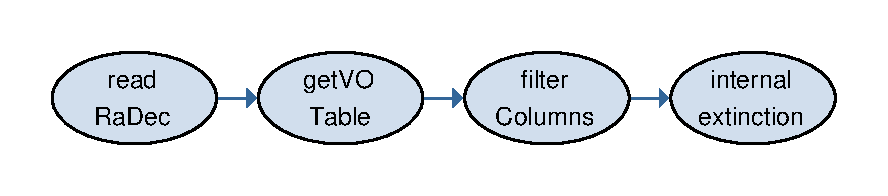
\includegraphics[width=.8\textwidth]{Figures/internal-extinction}
\caption{Pasos necesarios para el workflow internal extinction}\label{fig:internal}
\end{figure}

Nuestra investigación inicial sobre las dependencias para la ejecución de Internal extinction muestra que el software principal requeridos es el siguiente:  \verb|requests==2.20.0|, \verb|python=2.7.15=h33da82c_4|, \verb|numpy=1.15.0=py27h1b885b7_0| y \verb|astropy==2.0.9|


%todo: presentar los resultados




\subsubsection{Seismic Ambient Noise Cross-Correlation}


\textit{Seismic Ambient Noise Cross-Correlation workflow} (o xcorr workflow) es parte del proyecto \textit{Virtual Earthquake and seismology Research Community e-science environment in Europe} (VERCE).
Los terremotos y las erupciones volcánicas en ciertos casos van precedidos o acompañados de cambios en las propiedades geofísicas de la Tierra, como la velocidad de las olas o la velocidad de los eventos. El desarrollo de métodos fiables de evaluación de riesgos para estas amenazas requiere un análisis en tiempo real de los datos sísmicos y un pronóstico verdaderamente prospectivo y pruebas para reducir los sesgos. El objetivo del workflow es la prevision de riesgo a partir del pre procesamiento y correlación de forma cruzada las propiedades anteriores 
xcorr presenta dos etapas, la primera etapa es un preproceso donde cada serie de tiempo continua de una estación sísmica dada (llamada traza), está sujeta a una serie de tratamientos. El procesamiento de cada traza es independiente de otras trazas, haciendo que esta fase sea paralela y la segunda etapa empareja todas las estaciones y calcula la correlación cruzada para cada par. La figura \ref{fig:xcorr} muestra los pasos del workflow.



\begin{figure}[t]
\centering
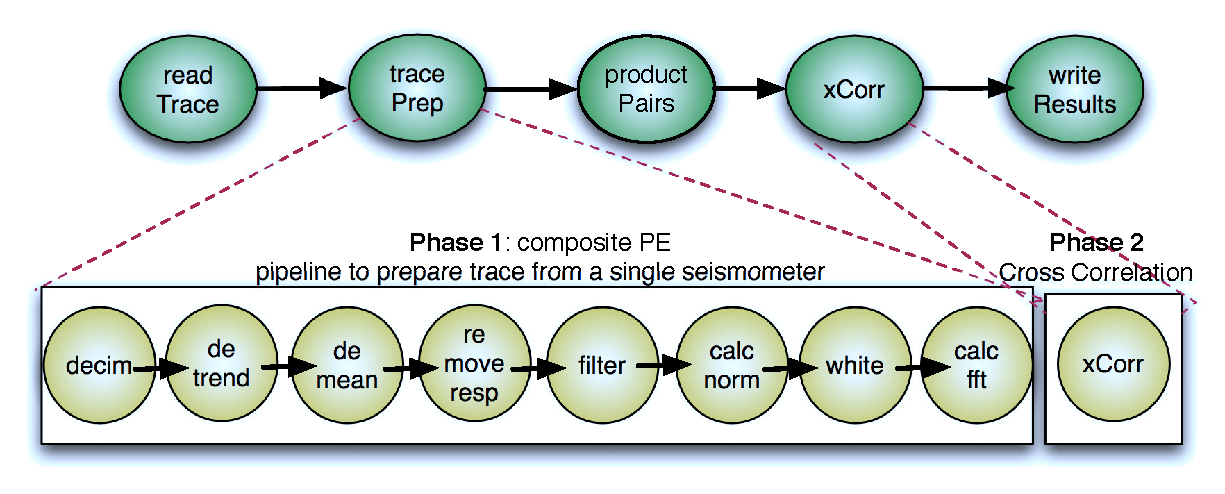
\includegraphics[width=.8\textwidth]{Figures/xcorr}
\caption{Pasos necesarios para el workflow internal extinction}\label{fig:xcorr}
\end{figure}


El software básico para la ejecución de Internal extinction es:  \verb|python=2.7.15=h33da82c_4|, \verb|obspy=1.1.0=py27h39e3cac_2| y \verb|numpy=1.15.0=py27h1b885b7_0|

%todo: presentar los resultados


\subsection{WINGS}

WINGS es un sistema de flujo de trabajo semántico que ayuda a los científicos en el diseño de experimentos computacionales. Un experimento computacional especifica cómo deben ser procesados los conjuntos de datos seleccionados por una serie de componentes de software en una configuración particular.
Los principales requisitos de pegasus son: Docker y Tomcat.
WINGS a diferencia de los otros sistemas de workflows utiliza imágenes Docker para su distribución. La imagen de sistema se encuentra disponible en \footnote{\url{https://hub.docker.com/r/dockerpedia/wings-docker/}}

Los principales requisitos de pegasus son: Java 1.8, Tomcat 8.5, Docker. La figura \ref{fig:pegasus-deps} muestra las dependencias especificadas tanto por el sistema de paquetes o documentación.

\begin{figure}[t]
\centering
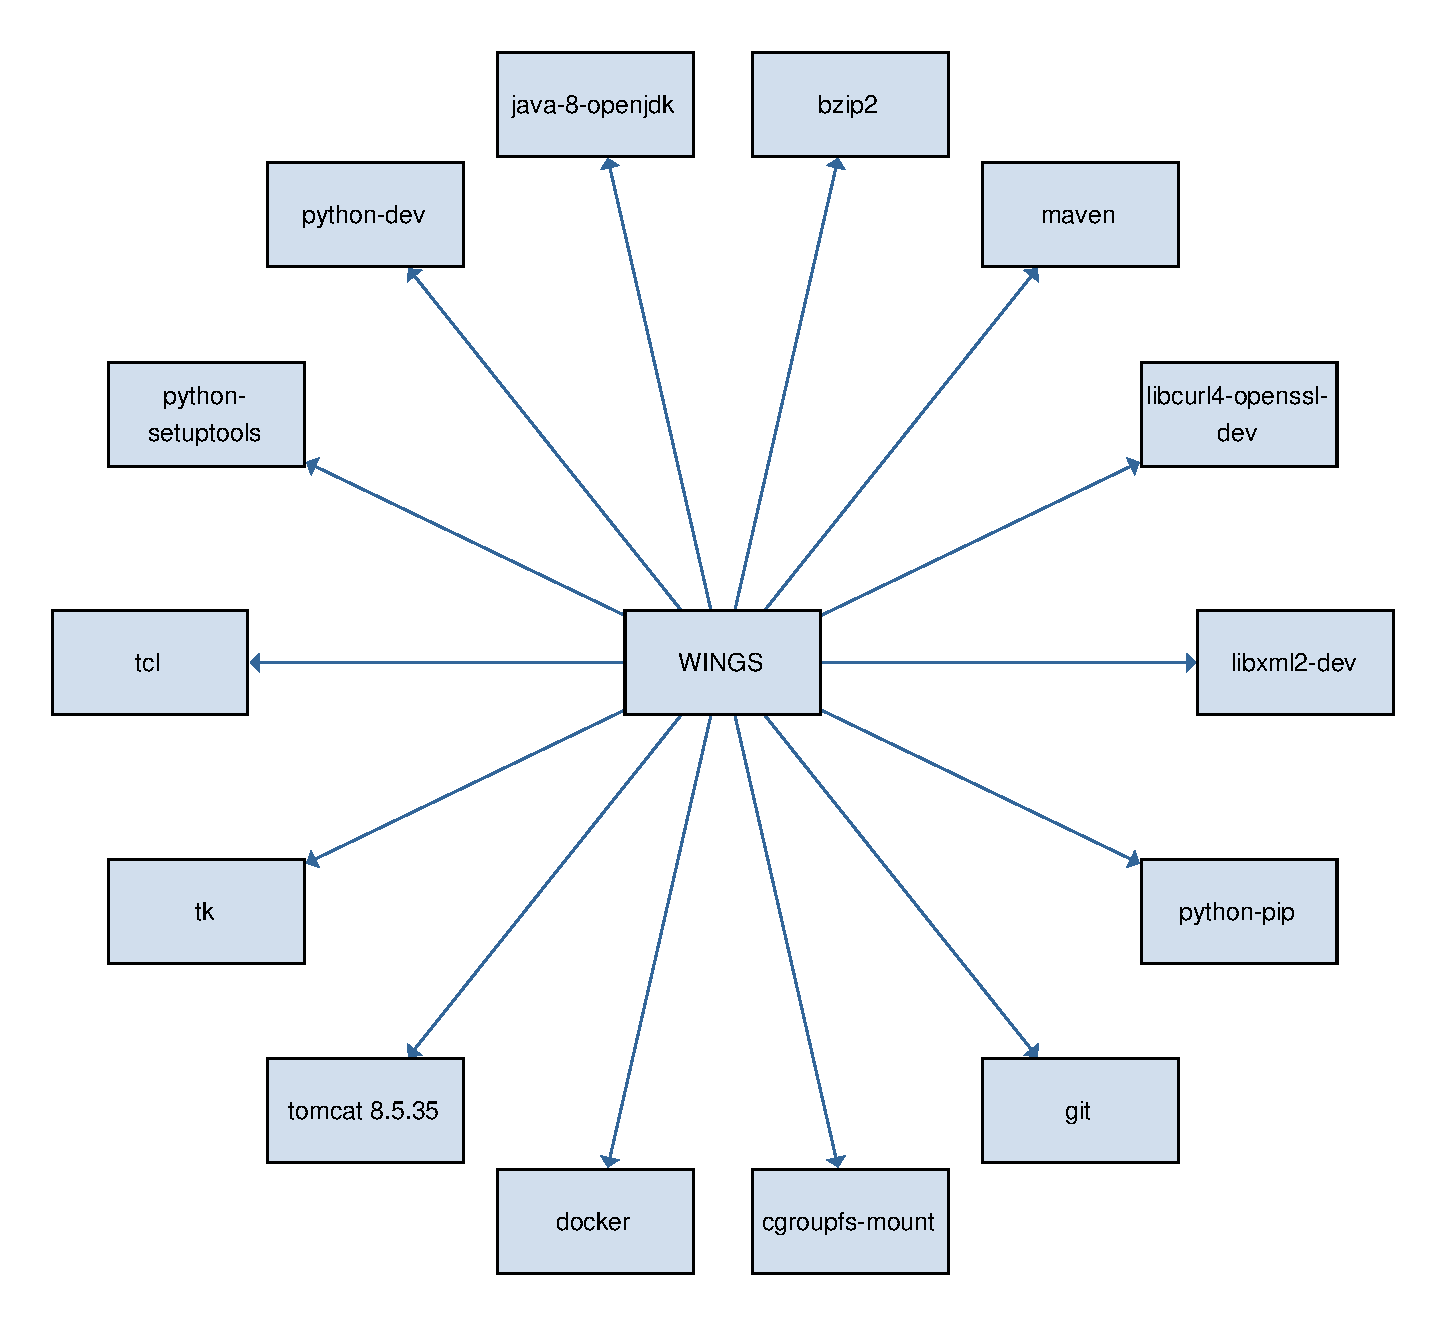
\includegraphics[width=.5\textwidth]{Figures/wings-deps}
\caption{Dependencias de WINGS}\label{fig:wigs-deps}
\end{figure}



Las imágenes se encuentran disponibles en DockerHub~\footnote{\url{https://hub.docker.com/r/dockerpedia/wings/}}


\subsubsection{MODFLOW-NWT}

MODFLOW es el modelo hidrológico modular del \textit{United Satatus Geological Survey} (USGS). MODFLOW se considera una norma internacional para simular y predecir las condiciones de las aguas subterráneas y las interacciones entre las aguas subterráneas y las aguas superficiales.
El USGS MODFLOW-NWT es una formulación de Newton-Raphson para MODFLOW-2005 para mejorar la solución de problemas de flujo de aguas subterráneas no confinadas. MODFLOW-NWT es un programa independiente destinado a resolver problemas de secado y rehumectación de las no linealidades de la ecuación de flujo de agua subterránea no confinada.


\begin{figure}[t]
\centering
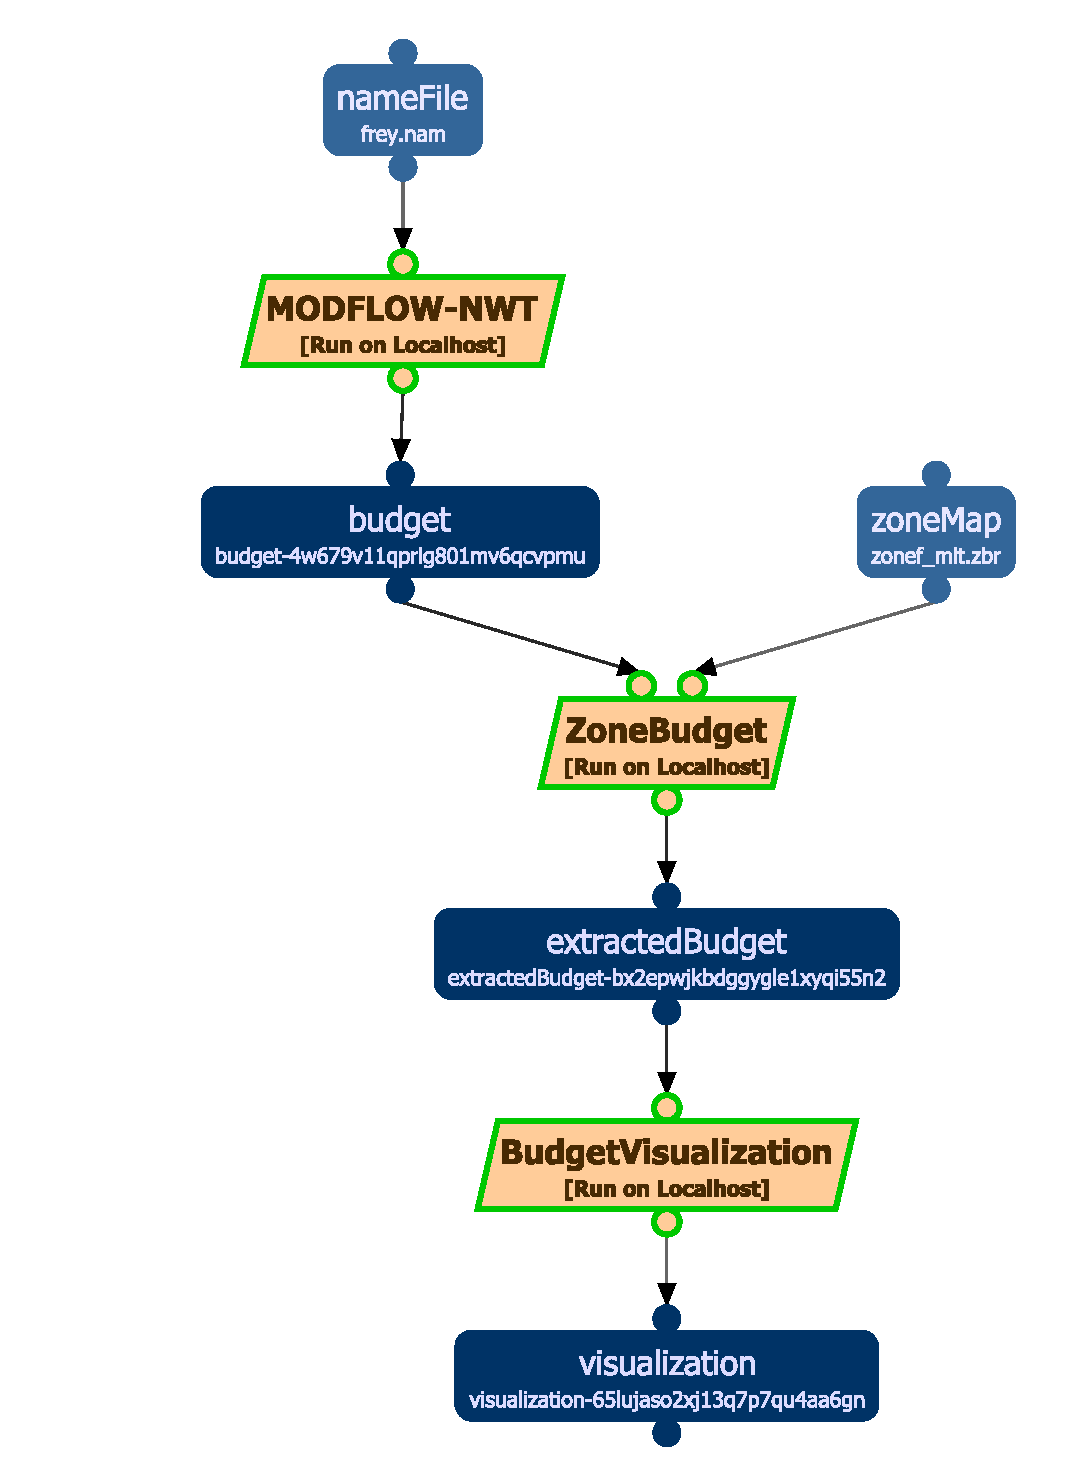
\includegraphics[width=0.6\textwidth]{Figures/usgs-modflow-nwt}
\caption{Figure caption.}\label{fig:modflow}
\end{figure}


La figura \ref{fig:modflow} muestra la estructura principal del worlklow, desarrollado con pipeline compuesto por tres pasos. El proceso inicia leyendo el modelo a utilizar. Luego, el archivo de zona se usa para especificar arreglos de zonas que van usarse y finalmente se genera una visualización que muestra la cantidad de millones de galones por día en zona. Las figuras \ref{fig:modflow-original} y \ref{fig:modflow-reproduced} muestran los resultados generados por el ambiente original y reproducido respectivamente.

\begin{figure*}[]
    \centering
    \begin{subfigure}[b]{\textwidth}
         \centering
         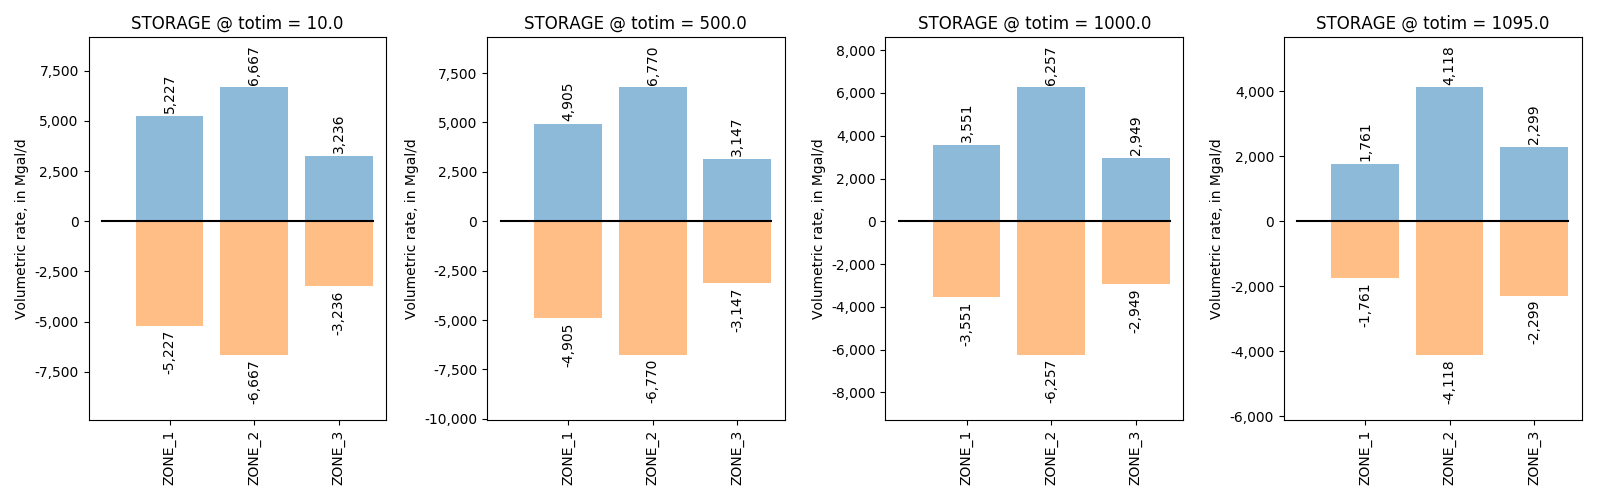
\includegraphics[width=\textwidth]{Figures/viz-original}
         \caption{Resultados originales entregados por el Information Sciences Institute}
         \label{fig:modflow-original}
     \end{subfigure}
	
	    \begin{subfigure}[b]{\textwidth}
         \centering
         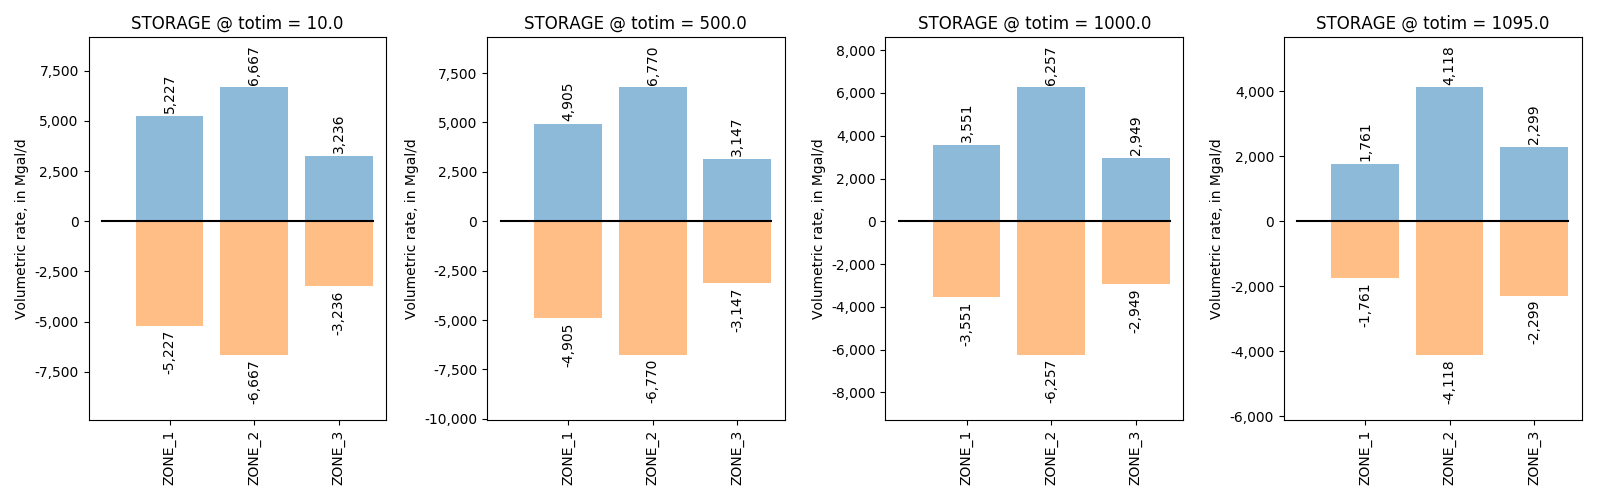
\includegraphics[width=\textwidth]{Figures/viz-reproduced}
         \caption{Resultados reproducidos por nuestra propuesta}
         \label{fig:modflow-reproduced}
     \end{subfigure}
        \caption{Los resultados obtenidos con el nuevo ambiente son iguales}
        \label{fig:both-modflow}
\end{figure*}






%-----------------------------------------------
% 5.2 Physical conservation
%-----------------------------------------------
\section{Conservación física}\label{s5.2}

Dado que publicamos las imágenes con su correspondiente Dockerfile, cualquier usuario puede inspeccionarlas y mejorarlas. Las imágenes puede ser encontradas en DockerHub \footnote{https://hub.docker.com/u/dockerpedia/} y \footnote{\url{https://github.com/dockerpedia}}. 

Para evaluar la conservación física utilizamos tres proveedores diferentes: DigitalOcean, Google Cloud y un local. La figura de \ref{image-env} presenta una descripción de las características de los ambientes    

\begin{table}[]
\centering
\begin{tabular}{|l|l|l|l|}
\hline
Resource   & Digital Ocean & Google Compute & Local     \\ \hline
RAM (GB)   & 8             & 8              & 4         \\ \hline
Disk (GB)  & 100           & 100            & 70        \\ \hline
CPU (GHz)  &               &                &           \\ \hline
CPU (Arch) & 64            & 64             & 64        \\ \hline
OS         & Centos 7      & Debian 9       & Fedora 27 \\ \hline
\end{tabular}
\caption{Image appliances characteristics.}
\label{image-env}
\end{table}

El ambiente debe tener instalado Docker, la información del manifiesto de la imagen de Docker describe la versión de Docker necesaria. Sin embargo, Docker asegura idempontencia para los ambientes CentOS7, Debian 10/9/8/7.7, Fedora 26/27/28, Ubuntu 14.04/16.06/18.04, Windows 10, macOS El Capitan 10.11 o nuevas versiones. El proceso de instalación puede ser encontrado en la documentación oficial \url{https://docs.docker.com/install/}

Cada imagen de Docker tiene archivo README con las instrucciones para correr el experimento. Las figuras \ref{lst:1}~\ref{lst:2} y~\ref{lst:3}  muestran los pasos necesarios para correr el experimento computacional. 

Para correr el experimento y descargar la imagen:

\begin{lstlisting}[caption={Descargar y correr la imagen disponible en DockerHub mosorio/pegasus\_workflow\_images:soykb},label={lst:1},language=bash]
docker run -d --rm -it --name soybean \
 mosorio/pegasus_workflow_images:soykb
\end{lstlisting}

Luego, el usuario debe entrar al container. El usuario puede confirmar que se encuentra dentro del container por el cambio de símbolo de la terminal  (prompt).

\begin{lstlisting}[caption={Entrar al ambiente computacional utilizando bash},label={lst:2},language=bash]
root@docker-instance:~# docker exec \
-ti -u workflow:workflow soybean bash
workflow@a0f861e6fbc4:~ 
\end{lstlisting}

Finalmente, correr el workflow. 

\begin{lstlisting}[caption={Run the workflow},label={lst:3},language=bash]
workflow@a0f861e6fbc4:~/soykb \
./workflow-generator --exec-env distributed	
\end{lstlisting}

Para evaluar si las imágenes Docker son livianas y almacenables, nosotros construimos dos imágenes, una utilizando Docker y otra utilizando máquinas virtuales. La imagen de Docker se construye bajo nuestro enfoque y la imagen de la máquina virtual basada en el trabajo de ~\cite{santana2017reproducibility}. Luego comparamos el uso de disco de ambas.



%-------------------------------------------
% Logical conservation
%-----------------------------------------------
\section{Conservación lógica}\label{s5.3}

A través de las anotaciones realizadas, buscamos describir los ambientes computacionales en forma automática, comparar las diferencias entre dos ambientes y construir un ambiente computacional similar que permita reproducir la ejecución del workflow. 

Para ello, anotamos los flujos de trabajo con nuestra herramienta, las anotaciones están agrupadas por: pasos de construcción y componentes de software. 

Para evaluar la calidad de las anotaciones utilizamos dos experimentos.

\begin{itemize}
	\item Reproducir el ambiente utilizando los pasos de construcción representados por DeploymentPlan
	\item Detectar las similitudes y diferencias entre dos ambientes computacionales usando distintas versiones de la distribución Linux.
\end{itemize}

Para obtener las anotaciones, proponemos usar Clair y construir un sistema de anotador. La figura \ref{fig:arch} muestra los pasos principales del sistema.


\begin{figure*}[]
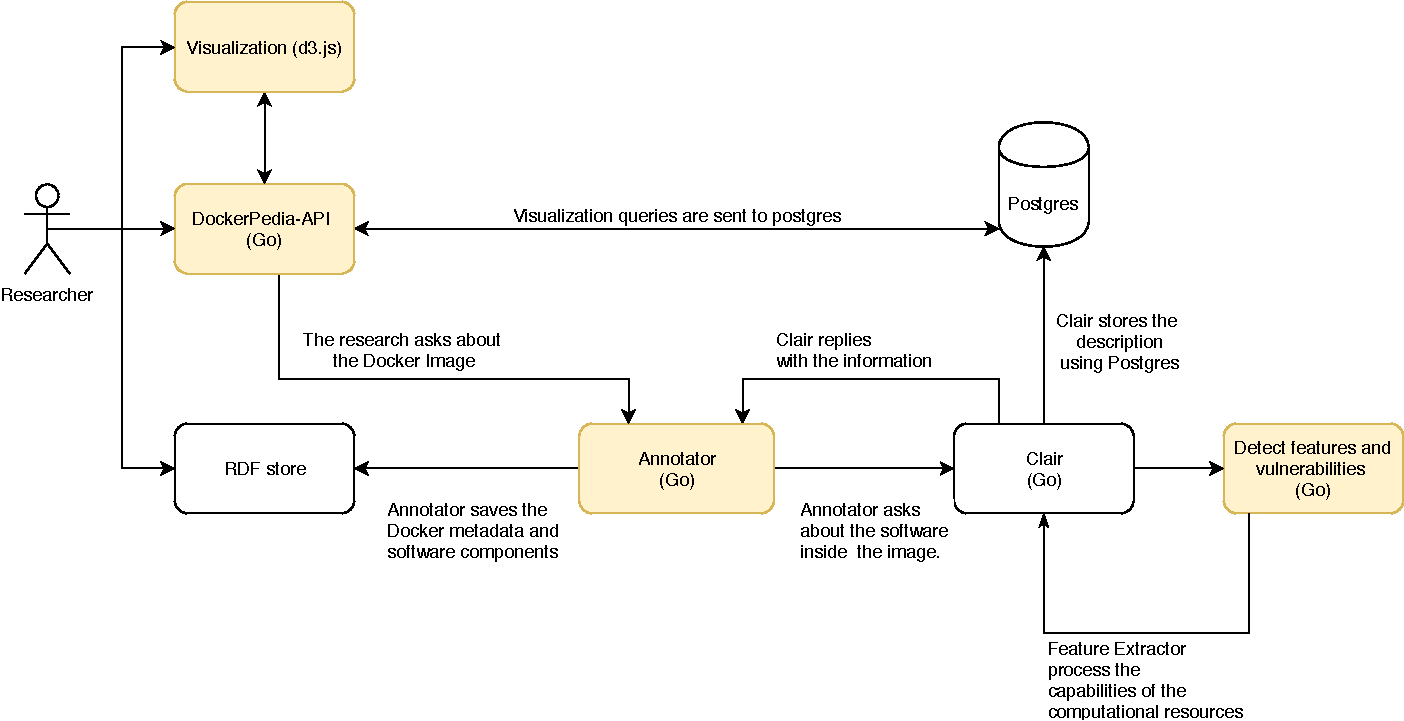
\includegraphics[width=\textwidth]{Figures/arch.pdf}
\caption{Figure caption.}\label{fig:arch}
\end{figure*}


\begin{enumerate}
    \item El investigador pregunta sobre la información de una imagen al sistema anotador. El sistema anotador se encuentra escrito en GoLang y disponible en nuestro repositorio.
    \item El sistema anotador pregunta a Clair sobre software y sus vulnerabilidades de la imagen. Nosotros utilizamos nuestra propia versión de Clair que puede detectar componentes de software instalado por Conda.
    \item Para obtener los pasos de construcción, etiquetas, arquitectura y más información. El anotador obtiene el manifiesto de la imagen desde DockerHub
    \item El sistema anotador guarda la información usando RDF y ontología propuesta.
\end{enumerate}


Para reproducir el entorno, el usuario debe clonar el repositorio y construir la imagen. La URL del repositorio y el cambio asociado (representado por un git commit) se pueden obtener por dos métodos: consultando nuestras anotaciones o usando un comando Docker. El listado \ref{lst:inspect_command} muestra las etiquetas de la imagen de flujo de trabajo SoyKB.


\begin{lstlisting}[caption={Inspect image annotations},label={lst:inspect_command},language=bash]
root@docker-instance:~# docker inspect \ 
    --format='{{json .Config.Labels}}' \ 
    dockerpedia/soykb:latest
\end{lstlisting}

La figura \ref{lst:inspect_result} muestra algunas de las etiquetas de la imagen basado en \textit{Open Container Initiative} 
\begin{lstlisting}[caption={Inspect image annotations},label={lst:inspect_result},language=json]
{
"maintainer": "Maximiliano Osorio <mosorio@inf.utfsm.cl>",
"org.label-schema.build-date": "2018-11-10T21:11:28Z",
"org.label-schema.name": "Soybean Knowledge Base",
"org.label-schema.schema-version": "1.0",
"org.label-schema.url": "http://www.soykb.org/",
"org.label-schema.vcs-ref": "15955b0",
"org.label-schema.vcs-url": "https://github.com/dockerpedia/soykb",
"org.label-schema.vendor": "DockerPedia",
"org.label-schema.version": "1.0"
}

\end{lstlisting}


Para evaluar si los entornos son similares, comparamos ambas imágenes utilizando el lenguaje de consulta SPARQL 1.1. El experimento fue un caso real en el que una imagen podía ejecutar el flujo de trabajo y la otra no. 
La figura \ref{lst:compare_query} muestra la consulta para identificar los diferentes componentes de software entre dos imágenes.

\begin{lstlisting}[caption={¿Cuáles son los diferentes componentes entre dos imágenes?},label={lst:compare_query},language=sparql]
SELECT * WHERE {
 pegasus_workflow_images%3Alatest
  vocab:containsSoftware ?p .
 MINUS{
 pegasus_workflow_images%3Apegasus-4.8.5
  vocab:containsSoftware ?p   
 }
}
\end{lstlisting}

\begin{lstlisting}[caption={¿Cuáles son los componentes que comparten entre dos imágenes?},label={lst:compare_query},language=sparql]
SELECT * WHERE {
 pegasus_workflow_images%3Alatest
      vocab:containsSoftware ?p .
 pegasus_workflow_images%3Apegasus-4.8.5
      vocab:containsSoftware ?p   
    }
    \end{lstlisting}
    
    
\section{Resultados y discusión}\label{s5.4}
Ejecutamos las imágenes sobre sus plataformas correspondientes. Aún mas, los componentes de software de la plataforma y la versión Docker son diferentes. Sin embargo, Docker garantiza que el software siempre funcionará de la misma manera, independientemente de dónde se instale.
Todas las ejecuciones se compararon con la original en una imagen VM predefinida, donde ya existía un entorno de ejecución.
Los resultados muestran que los ambientes de ejecución de contenedores son capaces de ejecutar completamente sus workflow relacionados. Para comprobar que no sólo los flujos de trabajo se ejecutan con éxito, sino también que los resultados son correctos y equivalentes, comprobamos los datos de salida producidos. 

Por otra parte, los resultados experimentales muestran que nuestra propuesta puede detectar automáticamente los componentes del software, las vulnerabilidades relacionadas, los pasos de construcción y los metadatos específicos de los experimentos científicos en forma de imágenes Docker. 
Además, los resultados muestran que es posible extender Clair para anotar a otros gestores de paquetes. 

Las anotaciones generadas por nuestro enfoque permiten comparar los componentes de software entre dos o más entornos. Esta función se puede utilizar como herramienta de depuración cuando un entorno reproducido no funciona.
Por ejemplo, en agosto de 2018, construimos la imagen del workflow SoyKB, y pudimos ejecutar el flujo de trabajo con éxito. Sin embargo, reconstruimos una nueva imagen en noviembre con el mismo DeploymentPlan y no se pudo ejecutar el workflow con éxito.


Describimos los componentes de software dentro de ambas imágenes. Y encontramos las siguientes diferencias:
\begin{itemize}
    \item Agosto: Pegasus 4.8 y Java 1.7
    \item Noviembre: Pegasus 4.9 y Java 1.8
\end{itemize}

Así, analizamos el código y la documentación de SoyKB y las dependencias de Pegasus 4.9. Como resultado, obtuvimos las gráficas de dependencia mostradas en la figura \ref{fig:pegasus49}.  Los gráficos de dependencia muestran que el paquete Pegasus 4.9 y SoyKB no son compatibles debido a sus requerimientos de versión Java.

Así, construimos una nueva imagen instalando Pegasus 4.8, y obtuvimos los gráficos de dependencia que se muestran en la figura \ref{fig:pegasus48}. Aquí, el gráfico no tiene un conflicto y se pudo ejecutar el workflow con éxito.


La nueva imagen fue nombrada como: \verb|pegasus_workflow_images:4.8.5|


\begin{figure*}[]
    \centering
    \begin{subfigure}[b]{0.40\textwidth}
         \centering
         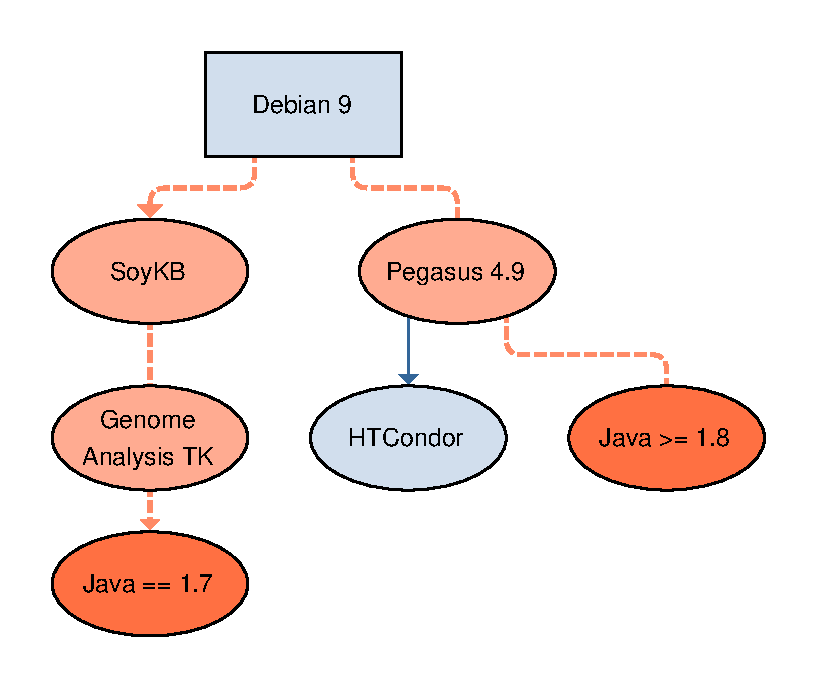
\includegraphics[width=\textwidth]{Figures/pegasus-49.pdf}
         \caption{Dependencies graph Pegasus 4.9 and SoyKB}
         \label{fig:pegasus49}
     \end{subfigure}
    ~ 
    \begin{subfigure}[b]{0.40\textwidth}
         \centering
         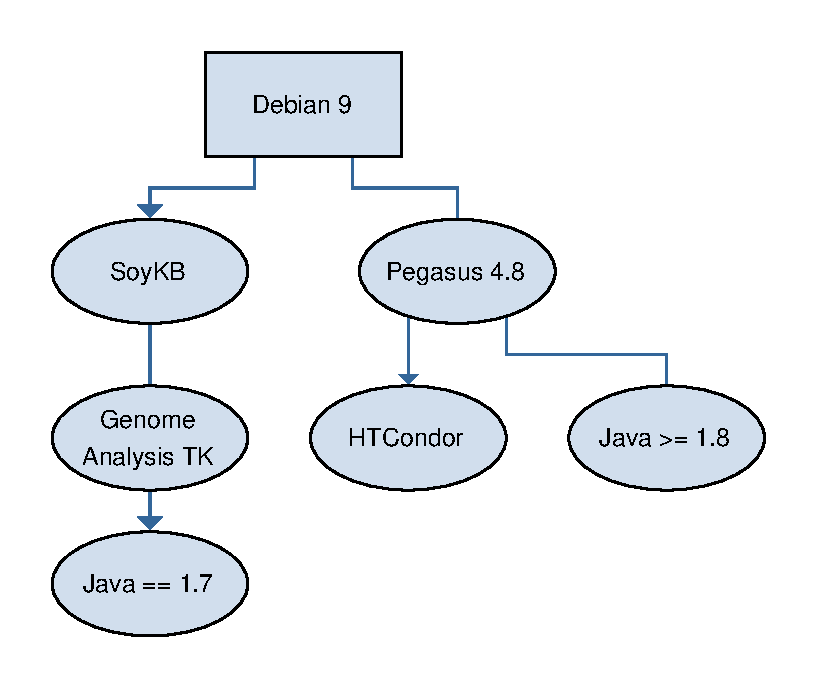
\includegraphics[width=\textwidth]{Figures/pegasus-48.pdf}
         \caption{Dependencies graph Pegasus 4.8 and SoyKB}
         \label{fig:pegasus48}
     \end{subfigure}
        \caption{The orange nodes are the differences between the images}
        \label{fig:dependencies-graph}
\end{figure*}


La razón principal de los trabajos anteriores para evitar la conservación física era la gran demanda de almacenamiento de máquinas virtuales. Afirmamos que las imágenes Docker son ligeras. 

Los resultados de la comparación del uso del disco muestran que hay una disminución del 64,2\% para la imagen Pegasus y del 41,5\% para la dispel4py. La tabla \ref{storage-reduce} muestra la diferencia para el sistema de flujo de trabajo Pegasus y dispel4py.


\begin{table}[]
\centering
\begin{tabular}{|l|l|l|}
\hline
Enfoque        & Pegasus (MB) & dispel4py (MB) \\ \hline
Virtualization & 1929         & 3509 \\ \hline
Container      & 690          & 2500 \\ \hline
\end{tabular}
\caption{Uso de disco de las imágenes pegasus y dispel4py utilizando máquinas virtuales y containers}
\label{storage-reduce}
\end{table}